\documentclass[10pt, a4paper]{article}
\usepackage{ictam}


\begin{document}

\title{TEMPLATE FOR ICTAM2020 SHORT PAPER (MAXIMUM 2 PAGES)}

\author[1]{\underline{Fabio Rossi}}
\author[1]{{Carlo Bianchi} {\footnote{Corresponding author. E-mail: ictam2020@aimgroup.eu.}}} 
%Corresponding author email should be added like this
\author[2]{Another Author}
\affil[1]{Department of Civil and Environmental Engineering, Politecnico di Milano, Milano, Italy}
\affil[2]{Department of Another Author, University of Another Author, City, Country}

\maketitle

\begin{abstract}
The following guidelines have been prepared for authors of papers to be presented at the forthcoming ICTAM2020 in Milano (Italy), 23-28 August 2020. They provide the rules for the preparation of short papers (maximum 2 pages), which will be used for selection by the International Papers Committee and for inclusion in the ICTAM2020 program. Authors are requested to follow these guidelines in order to achieve uniformity in the presentation of the Proceedings. This summary must not exceed 900 characters. Font Times New Roman for the whole manuscript, size 9 for this Summary and figures legends and captions, 10 for the whole manuscript. 
\end{abstract}

\section{MANUSCRIPT PREPARATION}
%\vspace{-2.5mm}

Congress participants are encouraged to submit papers from any area of theoretical and applied mechanics, especially those covered by the Thematic Sessions and the Mini-Symposia. The Congress website will be open for paper submission from 1 October, 2019. The deadline for paper submission is 10 January, 2020. Contributors will be informed of the decision of the International Papers Committee and of the assignment of their paper to a session before 10 April, 2020.

The paper must be in English, and should present material that is novel and preferably unpublished at the time of the Congress. All papers presented at the Congress are by invitation based on the recommendation of the International Papers Committee. No author will be invited to present more than one paper, with the exception that an author may present one paper on Education in Mechanics and another paper in one of the other sessions. Before submitting the paper you should register on the Congress website. Paper submission must be done electronically through the Congress website. The layout of the paper should follow the style of this document, starting with a title, followed by the name(s) of author(s) and affiliation(s).  \underline{The name of the author presenting the paper must be underlined}.


\subsection{Electronic submission of a Paper (PDF format)}

The paper will be used by the International Papers Committee as the sole mean of selection of papers for presentation at the Congress. All accepted papers will be published in the Congress program to be distributed to participants with other Congress materials. The paper is limited to a maximum of two A4 pages (including figures), and it must be submitted as a PDF document. The size of the PDF document must be less than 1 MB. \textbf{WHEN PREPARING THE PDF FILE REMEMBER TO EMBED ALL THE FONTS} into your PDF file; use TrueType fonts as much as possible, and avoid any special fonts.  If the reviewers cannot read your PDF file it is unlikely they will accept it!

The text should start with a title followed by the authors’ names and affiliations. The title should appear 20 mm below the top edge of the page. It should be brief, clear and descriptive. Use all bold capital letters centred on the width of the typing area. Leave one blank line after the title and another after the affiliation. A short summary (max. 900 characters) should be given at the beginning. If the paper is divided into sections and subsections, please adopt the format used here, in which the first-level headings are centred in bold capitals and the second level headings are left aligned in bold lower case letters, starting with a capital. Do not number sections. The text should be single-spaced using 10-point font. Begin paragraphs with 3 characters indentation at the left margin. The typing area of all pages should be 170 x 260 mm, leaving 20 mm margins on left, right, top and bottom. The total length of the paper, including all figures and references if any, cannot exceed two pages. The contribution should be prepared like a manuscript for journal submission.

All papers must be submitted online before Friday, 10 January, 2020.

\section{GENERAL GUIDELINES}
%\vspace{-2.5mm}

You are urged to make your paper as attractive as possible using text, figures, diagrams, and photographs. The paper will enable the reviewers and the International Papers Committee to decide upon the suitability of your contribution for the presentation at the Congress. It should specify the main assumptions, techniques and results, accompanied by background information about how your work relates to other works in the field. Only essential formulae and figures should be included and only key references need be given. A communicative title, a clearly presented summary and the main text will all assist the International Papers Committee in making a positive decision.

\section{ORAL PRESENTATION}
%\vspace{-2.5mm}

Papers accepted for the oral presentation will be arranged by subject into one of the parallel sessions. A period of 15 minutes, plus 5 minutes for discussion, will be allotted to each paper. Standard audio-visual presentation equipment will be available in each lecture room. Details regarding the Congress presentation facilities will be provided on the Congress website after May 15, 2020.

\section{SHORT TALK WITH POSTER PRESENTATION }
%\vspace{-2.5mm}
  Authors of papers accepted for short talk with poster presentation will be provided with an opportunity to make a short presentation during dedicated sessions. The time limit for this presentation is 5 minutes including change over. No questions will be permitted. The authors will be expected to stand by their posters during the poster session to respond to any potential questions. The Congress will provide poster boards and stands.
  
The usable area of a poster panel is 0.9m (width) by 1.2m (height). Authors are advised to read the details given on the Congress website. The recommended poster size is 841 mm wide x 1189 mm high (A0 vertical). Posters should be prepared directly on one sheet. The lettering should be large enough to be read by someone standing 2m back from the poster and the following text sizes are suggested. Title: 2-3 cm; Authors' names and affiliations: 2cm; Section headings (ABSTRACT, RESULTS, etc.): 2 cm. The text itself should be approximately 10mm high. The use of more diagrams, colour, and fewer words is recommended for clarity. Use phrases and short sentences in "bullet points". It is recommended that the poster be divided into the following sections: (i) summary; (ii) problem definition and/or goals; (iii) results and conclusions.


\begin{figure}[!t]
\centering
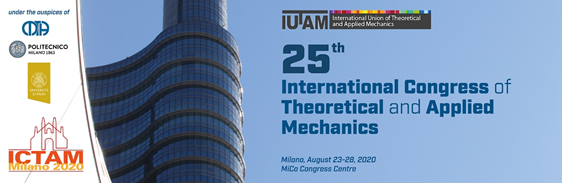
\includegraphics[width=6 in]{Figure.png}
\caption{\fontsize{9}{9}\selectfont Insert a figure caption, font size 9.}
\label{Fig1}
\end{figure}


\section{CONCLUSIONS}
%\vspace{-2.5mm}

Prepare the short paper as a PDF file, visit the ICTAM2020 web page, register (if you have not already done so), and submit the short paper following instructions on the web site. Confirmation will be sent to your e-mail address.


\begin{thebibliography}{9}
\bibitem{Ref1}
Cooler A. S. Binary Flow Systems. \textit{J. Fluid Mech.} \textbf{999}: 991-996, 1999.
\bibitem{Ref2}
Icer D. F., Adams J. A. Mathematical Elements for Computer Simulation. McGraw Hill, NY 1977.
\bibitem{Ref3}
Nygus G. Numerical Analysis Using Finite Element Method. \textit{PhD Thesis}, NTU Mech. Eng. Dept., Lagos, 1983.
\bibitem{Ref4}
ICTAM2020, web site \textbf{http://www.ictam2020.org}.
\end{thebibliography}

\end{document}
